\Problem{Suitcase Pull}{\SuitcasePull}{
	Using a handle at the end of a 15 kg suitcase, a boy is pulling it to the right across a rough horizontal floor with a force of 55 N at an angle of 25$ ^{\circ} $ above the horizontal. The force of kinetic friction between the suitcase and the floor is 75 N. Neglect air resistance and assume that the suitcase doesn’t leave the floor.
}

\ProblemSub{\SuitcasePullA}{
	(a) Draw a sketch showing the suitcase and the boy.
}
\Solution{\SuitcasePullASol}{
	\begin{figure}[h]
		\centering
		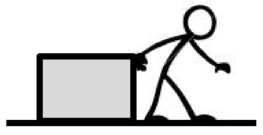
\includegraphics{\FileDepth/Activities/Suitcase_Pull/Boy_Pulling_Suitcase}
	\end{figure}
}
\ProblemSub{\SuitcasePullB}{
	(b) Identify the forces acting on the suitcase. For each force state whether it is a contact force or a long-range force.
}
\Solution{\SuitcasePullBSol}{The \textbf{force of gravity} is the only \textit{non-contact} force in this situation, pulling the suitcase toward the floor. To hold it up (at least partially), the floor exerts a \textbf{normal force} back on the suitcase, which is a \textit{contact} force. The floor also exerts a second \textit{contact} force on the suitcase: \textbf{kinetic friction}. The fourth and final force on the suitcase is \textbf{the boy's pull}, which is a \textit{contact} force. Since it is at an angle, some of it goes toward supporting the weight of the suitcase, which means the normal force does not have to be equal in magnitude to the force of gravity.
	
What type of force is the boy's pull? It depends on the choice of system. If the suitcase handle is not in the system with the suitcase, we might say we have a force of tension on the suitcase by the handle. In the more likely case that we include the handle in the system with the suitcase, then the boy's fingers are pushing on the inner surface of the handle, which would be a normal force. This is the choice I will make on the free body diagram.
}
\ProblemSub{\SuitcasePullC}{
	(c) Draw a free-body diagram for the suitcase. Use the particle model.
}
\Solution{\SuitcasePullCSol}{I will use the subscript $S$ (for ``surface'') to denote the floor, and $sc$ to denote the suitcase.
	
	Since the boy's pull exerts only 55 N at an angle of 25$ ^{\circ} $ above the horizontal, it will be overwhelmed by the oppositely oriented force of kinetic friction, which exerts 75 N horizontally on the suitcase:
	\[
	75 \text{ N} > (55\text{ N})\cos(25^{\circ}).
	\]
	Thus, the net force is to the left, and the suitcase is slowing down.
	\begin{figure}[h]
		\centering
		\begin{tikzpicture}
			\FBDaxes{0,0}{0}{axes}
			\FBDvectorMA{axes}{0.55}{25}{P}
			\node[anchor=west] at (Ptip) {$\vec{F}^{N}_{sc,B}$};
			\FBDvectorXY{axes}{-0.75,0}{FK}
			\node[anchor=south] at (FKtip) {$\vec{F}^{kf}_{sc,S}$};
			\FBDvectorXY{axes}{0,-1.5}{FG}
			\node[anchor=west] at (FGtip) {$\vec{F}^{g}_{sc,E}$};
			\FBDvectorXY{axes}{0,1.3}{FN}
			\node[anchor=west] at (FNtip) {$\vec{F}^{N}_{sc,S}$};
			\FBDvectorXY{2,0.5}{-0.25,0}{Fnet}
			\node[anchor=west] at (2,0.5) {$\vec{F}^{net}$};
		\end{tikzpicture}
	\end{figure}
}